\documentclass[10pt]{article}
\usepackage[polish]{babel}
\usepackage[utf8]{inputenc}
\usepackage[T1]{fontenc}
\usepackage{graphicx}
\usepackage[export]{adjustbox}
\graphicspath{ {./images/} }
\usepackage{amsmath}
\usepackage{amsfonts}
\usepackage{amssymb}
\usepackage[version=4]{mhchem}
\usepackage{stmaryrd}

\title{GIMNAZJUM }

\author{}
\date{}


\begin{document}
\maketitle
\begin{enumerate}
  \item Poniższą figurę potnij wzdłuż linii kratek na cztery identyczne części.\\
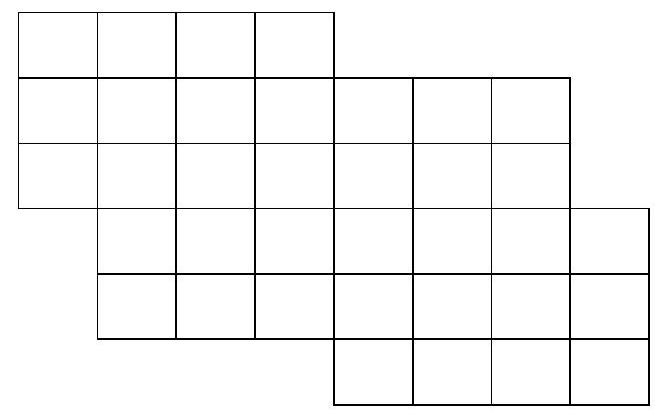
\includegraphics[max width=\textwidth, center]{2024_11_21_a1e3cfbefdcf841fc346g-1}
  \item Wstaw tak nawiasy, aby równość \(1-2 \cdot 3+4+5 \cdot 6 \cdot 7+8 \cdot 9=1995\) stała się prawdziwa.
  \item Uporządkuj rosnąco liczby: \(2^{45}, 3^{36}, 4^{27}, 5^{18}\),
\end{enumerate}

\section*{LICEUM}
\begin{enumerate}
  \item W trójkąt prostokątny \(A B C\) wpisano okrąg.
\end{enumerate}

Rzut tego okręgu na przeciwprostokątną AB jest odcinkiem MN. Wyznacz kąt MCN.\\
2. Rozwiąż rebus matematyczny wiedząc, że\\
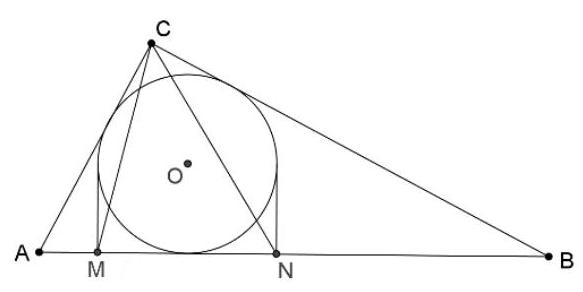
\includegraphics[max width=\textwidth, center]{2024_11_21_a1e3cfbefdcf841fc346g-1(1)}\\
jednakowym literom odpowiadają jednakowe cyfry, zaś różnym - różne.

\[
\begin{array}{r}
\text { SINUS } \\
\text { SINUS } \\
+ \text { KOSINUS } \\
\hline \text { TANGENS }
\end{array}
\]

\begin{enumerate}
  \setcounter{enumi}{2}
  \item Wiadomo, że \(a>b>0\) oraz \(a^{2}+b^{2}=6 a b\). Oblicz, ile wynosi \(\frac{a+b}{a-b}\).
\end{enumerate}

\end{document}